\authoredsection{Project Review}{Mohsin}{Mohsin Saeed}\label{sec:project-review}

\subsection{Challenges and Solutions}\label{sec:challenges}

The project faced three main practical constraints. Each was met with a deliberate workaround rather than a compromise on scope.

\subsubsection{No Dedicated Budget for Frontier Models}\label{sec:challenge-budget}

The pipeline depended heavily on language models. Stage 2 routing, the judge, and the optimizer all required repeated LLM calls, but the project had no budget allocated for frontier models. To keep development moving, we used Ollama to run open-source models locally. While this allowed us to build and test the pipeline without any cost, the available models were smaller and significantly slower than frontier models, making them unsuitable for large-scale judging and optimization experiments. Later in the project, we secured AWS Bedrock credits, providing access to models such as Claude Haiku and Claude Sonnet. This allowed us to combine the strengths of both approaches: Ollama for fast local development and Bedrock for the more demanding evaluation and optimization workloads. As a result, we were able to complete all experiments without incurring API costs.

\subsubsection{No Production Data}\label{sec:challenge-data}

Since Interhyp could not share production customer queries, there was no real-world dataset available for training or evaluating the pipeline. Instead, they provided the distribution of queries across the eight specialist agents, allowing us to construct datasets that reflected the expected workload. Rather than relying on a single dataset, we generated multiple datasets with increasing levels of difficulty, ranging from straightforward single-domain questions to complex multi-domain queries containing spelling mistakes and noisy copy-paste text. Evaluating the pipeline across this range provided a much clearer picture of its strengths and weaknesses than testing on only one type of data.

\subsubsection{An Inherently Complex System}\label{sec:challenge-complexity}

Unlike projects built around a single model, this one required several interconnected modules, the router, the judge, and the optimizer, each with its own logic but all needing to work together. Building this pipeline as one piece of software would have made debugging and testing far harder, so we used a modular architecture, developing and testing each component independently before integrating it. This kept the complexity manageable and let each part evolve without destabilizing the rest. The same complexity made the system hard to explain. With so many components interacting before a result appears, the full workflow was difficult to follow for anyone seeing it for the first time. To address this, we built a visual demonstration showing a query moving through each stage, and used a football analogy in the presentation to explain each component's role. This made the system easier to follow while still accurately representing its underlying complexity.

\subsection{Limitations}\label{sec:limitations}

While the project achieved its intended goals, several limitations remain due to the scope of the evaluation and the constraints under which the system was developed.

The most significant limitation is that the evaluation relied entirely on synthetic data. Although the datasets were designed based on the query distribution across the eight agents and deliberately covered different levels of difficulty, they can only approximate real broker traffic. The system was never evaluated with live user queries. Therefore, the reported accuracy values should be interpreted as promising but not yet representative of production performance. The pipeline's long-term behavior, performance under real traffic, and production latency still need to be validated on real data.

A second limitation is that the self-improvement loop relies on a single judge. While the judge currently achieves 99\% agreement with the ground truth, this does not mean it is guaranteed to be error-free. The concern is structural: because every correction to the router comes from this one component, its mistakes have nowhere to be caught. Any error the judge makes would feed straight into the Stage 1 store and the optimizer and shape the router from there.

Finally, the pipeline was evaluated on a limited range of models: local models served through Ollama, and Claude Haiku and Claude Sonnet through Bedrock. The behavior of the system may differ when using other providers, model families, or model sizes. Therefore, the findings are limited to the specific models and configurations evaluated in this project.

\subsection{Potential Enhancements}\label{sec:enhancements}

The project established several directions for future improvement. Two of these enhancements were already explored during the final sprint, while the remaining opportunities build on limitations identified during evaluation.

\subsubsection{Monitoring Dashboard}\label{sec:enhancement-dashboard}

To give Interhyp visibility into the system in production, the team built a monitoring dashboard (\cref{fig:monitoring-dashboard}). It provides a single view of key system metrics, including router accuracy, query volume, the proportion of queries resolved directly by Stage 1, average latency, and LLM costs. The dashboard and supporting data pipeline are already implemented; however, it currently displays demo data because the system has not yet received live traffic. Every chart would fill with real data automatically once queries begin to flow. The remaining step is deploying it against live production traffic, at which point it would let Interhyp track accuracy, cost, and index growth over time and catch drift or regressions early, closing the gap left by evaluating the system only offline.

\begin{figure}
\centering
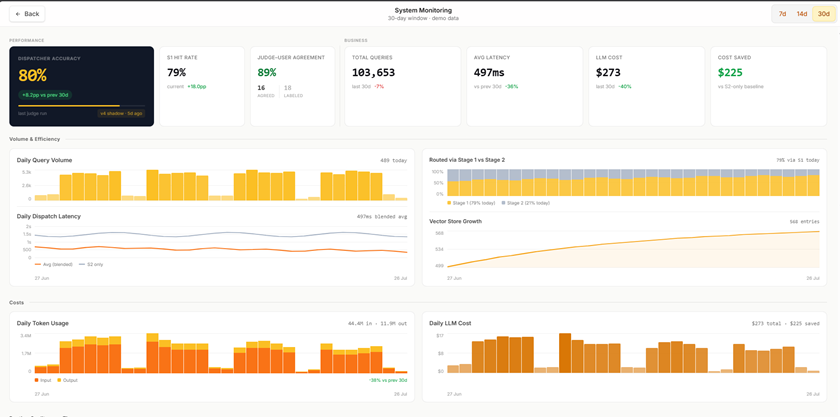
\includegraphics[width=0.85\linewidth,height=\textheight,keepaspectratio]{assets/review/monitoring-dashboard.png}
\caption{The monitoring dashboard, shown with demo data pending live traffic, giving a single operator-facing view of accuracy, the Stage 1 and Stage 2 routing split, latency, volume, vector-index growth, and cost.}\label{fig:monitoring-dashboard}
\end{figure}

\subsubsection{Human in the Loop}\label{sec:enhancement-hitl}

The judge currently provides the feedback signal that drives the improvement loop without human verification. A human-in-the-loop approach would introduce human validation alongside the automated judge. The team sketched a concept for this (\cref{fig:human-in-the-loop}): an interface that presents two candidate answers side by side so a reviewer can choose the more helpful one, extended in future by a lightweight thumbs up or down control on individual answers. Signals collected this way would give an independent check on the judge's verdicts and a source of high-confidence labels, so the automated judge is no longer the only source of truth. This remains a proposed design rather than an implemented feature.

\begin{figure}
\centering
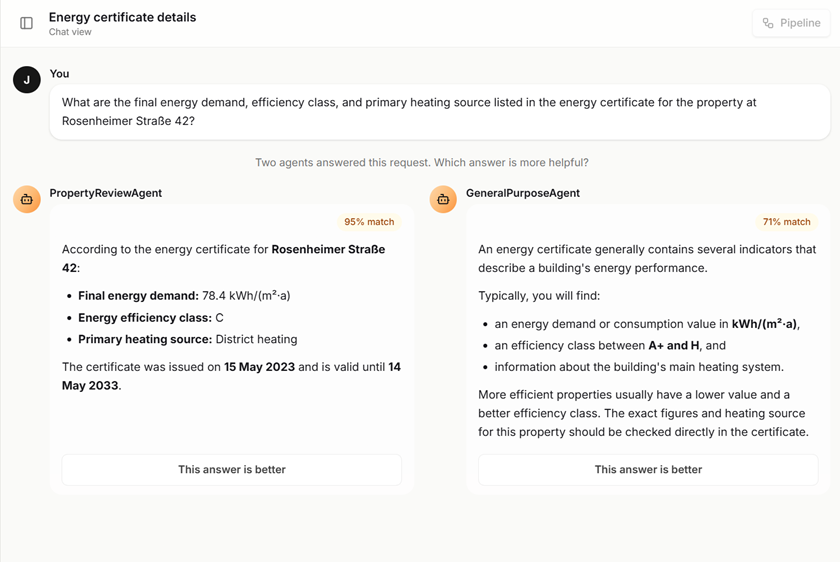
\includegraphics[width=0.85\linewidth,height=\textheight,keepaspectratio]{assets/review/human-in-the-loop.png}
\caption{Concept design for a human-in-the-loop review step, in which a reviewer selects the more helpful of two answers. Proposed, not yet implemented.}\label{fig:human-in-the-loop}
\end{figure}

\subsubsection{Hyperparameter Tuning}\label{sec:enhancement-hyperparameters}

Several values in the current system are manually configured, the number of candidate agents the judge compares, and optimizer settings such as the number of rounds and candidates. These values could instead be treated as tunable hyperparameters and optimized using Interhyp's own data and objectives. This would allow the system to be calibrated according to their priorities, balancing accuracy, latency, and cost rather than relying on values selected under the project's time constraints.

\subsubsection{Judge}\label{sec:enhancement-judge}

As the limitations already indicated, although the judge reached 99\% agreement on the evaluation dataset, it is not guaranteed to be error free on new production queries. It will be required in the future to test the judge's reliability periodically with a ground truth dataset constructed out of new queries. If the judge agreement rate on this dataset drops significantly, setting up a judge panel would be the most reasonable next step.

Furthermore, we investigated using the judge model's log probabilities as a confidence signal to quantify how certain the judge was about a given verdict rather than only obtaining a binary decision and its reasoning. Such a signal could be compared against the router's own confidence in its routing decision to estimate the size of the resulting error signal or used to flag particularly uncertain cases for human review, strengthening the human-in-the-loop approach. This did not prove feasible with GPT-OSS-120B, the model used for this exploration via the AWS Bedrock API. As a reasoning model, it commits to its decision internally before generating the visible output token, so the extracted log probabilities were consistently 100\% for one candidate and 0\% for the other, regardless of how close the actual decision was. The approach may still be viable with non-reasoning models that expose meaningful log probabilities, and remains worth revisiting when different models are available.
